%  This LaTeX template is based on T.J. Hitchman's work which is itself based on Dana Ernst's template.  
% 
% --------------------------------------------------------------
% Skip this stuff, and head down to where it says "Start here"
% --------------------------------------------------------------
 
\documentclass[12pt]{article}
 
\usepackage[margin=1in]{geometry} 
\usepackage{amsmath,amsthm,amssymb}
\usepackage{graphicx}
\usepackage{siunitx,ifthen}
\usepackage{bbold}
\usepackage{tikz}
\usepackage{hyperref}
\usepackage{gensymb}
\usepackage{amsfonts}
\usepackage{blindtext}
\usepackage{titlesec}
\usepackage{mathtools}
\DeclarePairedDelimiter{\ceil}{\lceil}{\rceil}
\newcommand{\tderiv}{{\frac{\rm{d}}{\rm{d}t}}}

\newcommand{\tsderiv}{{\frac{\rm{d}^2}{\rm{d}t^2}}}

\newenvironment{statement}[2][Statement]{\begin{trivlist}
\item[\hskip \labelsep {\bfseries #1}\hskip \labelsep {\bfseries #2.}]}{\end{trivlist}}

\begin{document}
 
% --------------------------------------------------------------
%
%                         Start here
%
% --------------------------------------------------------------
 
\title{TSA 1 Problem Set (God \LaTeX was a mistake, I'm doing the next one pencil and paper)} % replace with the problem you are writing up
\author{Grant Yang} % replace with your name
\maketitle

\tableofcontents
\newpage

\section{Textbook Problems}
% \begin{itemize}
%     \item HRW Chapter 2: Problems 3, 14, 22, 31, 46
%     \item HRW Chapter 4: Problems 14, 20, 55, 69, 97
% \end{itemize}
 
\subsection{Problem 2.3}
An automobile travels on a straight road for
40 km at 30 km/h. It then continues in the same direction for another 40 km at 60 km/h.

\paragraph{Part A} 
What is the average velocity of the car during the full 80 km trip? (Assume that it moves in the positive x direction.) \newline

1-dimensional motion with constant velocity is given by \begin{equation}\Delta x = v_x \Delta t. \label{eq1}\end{equation}

Thus, to calculate the total time this trip takes, we can break it up into its two segments and write this equation:
\[\Delta t_\text{total} = \frac{40\,\si{km}}{30\,\si{kph}} + \frac{40\,\si{km}}{60\,\si{kph}} = 2\,\si{h}.\]

To calculate average velocity, we take equation \eqref{eq1} but instead take $\Delta x_\text{total} = v_\text{avg} \Delta t_\text{total}$:

\[v_\text{avg} = \frac{\Delta x_\text{total}}{\Delta t_\text{total}} = \frac{80\,\si{km}}{2\,\si{h}} = \boxed{40\,\si{kph}}\]


\paragraph{Part B} What is the average speed? \newline

Because this is one dimensional motion and it never changes direction, the average speed is equal to the average velocity:

\[s_\text{avg} = v_\text{avg} = \boxed{40\,\si{kph}}\]

% \newpage
\begin{figure}[h]
\centering
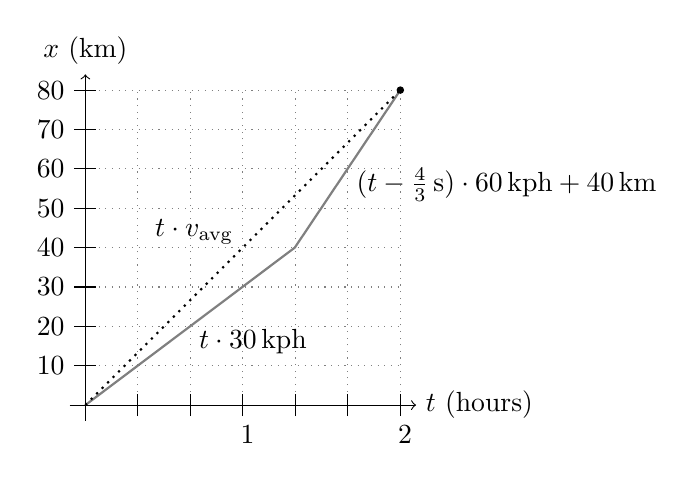
\begin{tikzpicture}[scale=2]
\foreach \x [evaluate=\x as \lab using int(\x*10)] in {1,2,...,8}
{
    \draw[dotted,gray] (0, {\x/4}) -- (2, {\x/4}); 
    \draw (-0.07, {\x/4}) -- (0.07, {\x/4}) (-0.07,{\x/4}) node[anchor=east] {\lab};
}
\foreach [
    evaluate=\b as \y using \b/3,
    evaluate=\b as \num using {int(mod(\b,3))},
    evaluate=\b as \iy using int(\b/3)] \b in {1,2,...,6}
{
    \draw[dotted,gray] ({\y}, 0) -- ({\y}, 2); 
    \draw ({\y}, -0.07) -- ({\y}, 0.07) ({\y}, -0.07) node[anchor=north] {\ifthenelse{\equal{\num}{0}}{
    \pgfmathprintnumber[fixed, precision=2]{\y}}{}};
}
\draw[thick,gray] (0,0) -- (1.33, 1) -- (1.33, 1) -- (2, 2);
\draw (1.66, 1.4) node[anchor=west] {$(t-\frac{4}{3}\,\si{s})\cdot 60\,\si{kph}+40\,\si{km}$};
\draw[fill] (2,2) circle[radius=0.02];
\draw[thick,dotted] (0,0) -- (2,2);
\draw (1, 1.1) node[anchor=east] {$t \cdot v_\text{avg}$};
\draw[->] (-0.1,0) -- (2.1,0);
\draw[->] (0,-0.1) -- (0,2.1);
\draw (2.1,0) node[anchor=west] {$t$ (hours)} (0, 2.1) node[anchor=south] {$x$ (km)};
\draw (0.66, 0.4) node[anchor=west] {$t\cdot 30\,\si{kph}$};
\end{tikzpicture}
\caption{\textbf{Part C} Graph x versus t and indicate how the average velocity is found on the graph.}
\end{figure}

\subsection{Problem 2.14}
An electron moving along the x axis has a position given by $x=16t e^{-t}\,\si{m}$, where t is in seconds. How far is the electron from the origin when it momentarily stops? \newline

First, we solve for time when velocity is zero:
\[0 = v = \dot x = 16 e^{-t} (1 - t)\] %\frac{\text{d}x}{\text{d}t}

Because $e^{-t} > 0$ for all real $t$, the electron must only stop at $t=1\,\si{s}$. At that time, it is at $x = 16 e^{-1}\,\si{m} \approx 5.9\,\si{m}$. The electron is \fbox{5.9 meters from the origin.}

\subsection{Problem 2.22}
The position of a particle moving along the x axis depends on
the time according to the equation $x = c t^2 - bt^3$, where x is in meters and t in seconds.

\begin{itemize}
\item[] \textbf{Part A\:} The units of $c$ are $\boxed{\si{m \cdot s^{-2}}}$
\item[] \textbf{Part B\:} The units of $b$ are $\boxed{\si{m\cdot s^{-3}}}$
\end{itemize}

Let $c = 3.0\,\si{m \cdot s^{-2}}$ and $b = 2.0\, \si{m\cdot s^{-3}}$.

\paragraph{Part C}  At what time does the particle reach its maximum positive x position? \newline

%By inspection, we see that $x \to -\infty$ as $t \to -\infty$ and $x \to \infty$ as $t \to \infty$. 
To find the maximum of $x$, we take its first and second derivatives:

\begin{equation}
    \dot x = 2 c t - 3 b t^2 \label{vel22}
\end{equation}
\begin{equation}
    \ddot x = 2 c - 6 b t \label{accel22}
\end{equation}



The first derivative is $0$ when $t \in \{0, \left.{2c}\middle/{3b}\right.\}$. However, only at $t =\left.{2c}\middle/{3b}\right.$ do we have a maximum as $\ddot x < 0$ (assuming $c > 0$). At $t=0$, $\ddot x > 0$ and we have a minimum. Thus, the maximum positive x position is achieved at:

\[
t = \frac{2 c}{3 b} = \frac{6.0\,\si{m \cdot s^{-2}}}{6.0\,\si{m\cdot s^{-3}}} = \boxed{1.0\,\si{s}}
\] \newline

Next, let us examine the time interval from t = 0.0 s to t = 4.0 s.

\paragraph{Part D}
The distance a particle moves is the time integral of the magnitude of its velocity:
\[
\int |\dot x|\,\rm{d}t
\]

Examining the sign of $\dot x$, we see that it is positive if $0 < t < 2c/3b$ and negative otherwise. Because $2c/3b = 1.0\,\si{s}$, the integral becomes:
\begin{align*}
\int |\dot x|\,\rm{d}t&=\int_{0.0\,\si{s}}^{1.0\,\si{s}} \left[(6.0\,\si{m\cdot s^{-2}}) t - (6.0\,\si{m\cdot s^{-3}})t^2\right]\rm{d}t 
    \\&\quad+ \int_{1.0\,\si{s}}^{4.0\,\si{s}} \left[(6.0\,\si{m\cdot s^{-3}})t^2 - (6.0\,\si{m\cdot s^{-2}}) t\right]\rm{d}t
\\&= 6.0\,\si{m} \Big[\frac{1}{2\,\si{s^2}}t^2-\frac{1}{3\,\si{s^3}}t^3\Big|^{1.0\,\si{s}}_{t=0.0\,\si{s}} + 6.0\,\si{m} \Big[\frac{1}{3\,\si{s^3}}t^3-\frac{1}{2\,\si{s^2}}t^2\Big|^{4.0\,\si{s}}_{t=1.0\,\si{s}}
\\&\approx \boxed{82\,\si{m}}
\end{align*}

\paragraph{Part E} Displacement can be calculated by 
\begin{align*}
\Delta x &= x_\text{final} - x_\text{initial}
\\&= \left[(3.0\,\si{m\cdot s^{-2}}) (4.0\,\si{s})^2 - (2.0\,\si{m\cdot s^{-3}}) (4.0\,\si{s})^3\right] - 0\,\si{m}
\\&\approx \boxed{-80\,\si{m}}
\end{align*}

\paragraph{Parts F through I}
Looking at equation \eqref{vel22}, we get
\[
v = \dot x = (6.0\,\si{m\cdot s^{-2}}) t - (6.0\,\si{m\cdot s^{-3}}) t^2
\]

\fbox{
\begin{tabular}{c|c}
    $t$ & $v$ \\
    \hline
    1.0 s & $0\,\si{m\cdot s^{-1}}$\\
    2.0 s & $-12\,\si{m\cdot s^{-1}}$\\
    3.0 s & $-36\,\si{m\cdot s^{-1}}$\\
    4.0 s & $-72\,\si{m\cdot s^{-1}}$\\
\end{tabular}
}

\paragraph{Parts J through M}
Looking at equation \eqref{accel22}, we get
\[a = \ddot x = (6.0\,\si{m\cdot s^{-2}}) - (12\,\si{m\cdot s^{-3}}) t\]

\fbox{
\begin{tabular}{c|c}
    $t$ & $a$ \\
    \hline
    1.0 s & $-6\,\si{m\cdot s^{-2}}$ \\
    2.0 s & $-18\,\si{m\cdot s^{-2}}$ \\
    3.0 s & $-30\,\si{m\cdot s^{-2}}$\\
    4.0 s & $-42\,\si{m\cdot s^{-2}}$ \\
\end{tabular}
}

\newpage
\subsection{Problem 2.31}
Suppose a rocket ship in deep space moves with constant acceleration equal to $9.8\,\si{m/s^2}$, which gives the illusion of normal gravity during the flight. 

\paragraph{A.} Light travels at $3.0 \times 10^8\,\si{m/s}$. How long does it take to accelerate from rest to $0.1c$?
\[
\Delta v = a \Delta t
\]
\[
0.1c = 9.8\,\si{m/s^2} \Delta t
\]
\[
\Delta t = \frac{0.1 \times 3.0 \times 10^8\,\si{m/s}}{9.8\,\si{m/s^2}} \approx \boxed{3.1 \times 10^6\,\si{s}}
\]

\paragraph{B.} Using the definitions of position, velocity, and acceleration:
\[
\Delta x = v_0 \Delta t + \frac{1}{2} a \Delta t^2
\]

Plugging in that we start at rest from $v_0 = 0$, we can calculate
\[
\Delta x = \frac{1}{2} \left(9.8\,\si{m/s^2}\right)\left(3.1\times10^6\,\si{s}\right)^2 \approx \boxed{4.6\times10^{13}\,\si{m}}
\]

Thus, over the course of about 35 days, we accelerate to 0.1c and travel about 307 astronomical units.

\subsection{Problem 2.46}
Raindrops fall 1700 m from a cloud to the ground. 

\paragraph{A.} If they were not slowed by air resistance, how fast would the drops be moving when they struck the ground? \newline

Assuming zero initial velocity ($v_0 = 0$) and that the positive x direction represents falling downwards:
\[
\Delta x = \frac{1}{2} a \Delta t^2
\]
\[
\Delta t = \sqrt{\frac{2 \Delta x}{a}}
\]
\begin{align*}
\Delta v &= a \Delta t 
\\&= a \sqrt{\frac{2 \Delta x}{a}} =  \sqrt{2 a \Delta x}
\\&=\sqrt{2 (9.8\,\si{m/s^2}) (1700\,\si{m})} \approx \boxed{183\,\si{m/s}}
\end{align*}

\paragraph{B.} Without air resistance, it would probably not be safe to walk outside in a rainstorm. If rain in a heavy shower falls at a rate of \href{https://water.usgs.gov/edu/activity-howmuchrain-metric.html}{$10\,\si{mm/h}$} and that water has a density of $1\,\si{g/cm^3}$, we can calculate the energy intensity (energy per area) of the rain using $E_k = \frac{1}{2} m v^2$:

\[
\frac{1}{2} (10\,\si{\tfrac{mm}{h}})(1\,\si{\tfrac{g}{cm^3}})(183\,\si{\tfrac{m}{s}})^2 = 46.5\,\si{W/m^2}
\]

I don't know what level of discomfort that translates to but that is probably not good. If an individual raindrop were \href{https://www.wolframalpha.com/input?i=mass+of+raindrop&assumption=%7B%22F%22%2C+%22RaindropProperties%22%2C+%22d%22%7D+-%3E%224+mm%22}{34 milligrams}, it would have an energy of about 0.5 Joules. That is equivalent to a \href{https://www.wolframalpha.com/input?i=mass+of+baseball}{145 gram} baseball hitting you at 6.3 mph. Being pelted with baseballs going decently fast is not ideal.

\subsection{Problem 4.14}
A proton initially has $\vec{v} = 4.0 \hat{i} - 2.0\hat{j} + 3.0\hat{k}$ and then 4.0 s later has $\vec{v} = -2.0\hat{i}-2.0\hat{j}+5.0\hat{k}$ (in meters per second). For that 4.0 s:

\paragraph{A.} The average acceleration was
\begin{align*}\vec{a}_\text{avg} &= \frac{\vec{v}_\text{final} - \vec{v}_\text{initial}}{\Delta t} = \frac{(-2.0\hat{i}-2.0\hat{j}+5.0\hat{k}) - (4.0 \hat{i} - 2.0\hat{j} + 3.0\hat{k})}{4.0\,\si{s}}\\&= \boxed{-1.5\hat{i} + 0.5\hat{k}\quad(\si{m/s^2})}\end{align*} 

\paragraph{B.} The magnitude of $\vec{a}_\text{avg}$ is:
\[|| \vec{a}_\text{avg} || = \sqrt{(-1.5)^2 + (0.5)^2} = \sqrt{3.5} \approx \boxed{1.58\quad(\si{m/s^2})}\]

\paragraph{C.} Because the dot product $\vec{a}\cdot\vec{b} = \lvert\lvert \vec{a}\rvert\rvert\,\lvert\lvert \vec{b}\rvert\rvert \cos{\theta}$ where $\theta$ is the angle between them, the angle between $\vec{a}_\text{avg}$ and the positive direction of the x axis is:
\[\cos^{-1}\left(\hat{i}\cdot \frac{\vec{a}_\text{avg}}{||\vec{a}_\text{avg}||}\right) \frac{180\degree}{\pi\,\si{rad}}\approx \boxed{162\degree}\]

\newpage
\subsection{Problem 4.20}
Particle A moves along the line $y = 30\,\si{m}$ with a constant velocity $\vec{v}$ of magnitude $3.0\,\si{m/s}$ and parallel to the x axis. At the instant particle A passes the y axis, particle B leaves the origin with a zero initial speed and a constant acceleration $\vec{a}$ of magnitude $0.40\,\si{m/s^2}$. What angle $\theta$ between $\vec{a}$ and the positive direction of the y axis would result in a collision? \newline

Let $a$ be the magnitude of the acceleration. We can parametrize the positions of A and B as:
 \[
\vec{x}_A = \begin{bmatrix}vt \\ y_0\end{bmatrix} \qquad\qquad \vec{x}_B = \frac{1}{2} a \begin{bmatrix}\sin(\theta) \\ \cos(\theta) \end{bmatrix} t^2
\]

Setting $\vec{x}_A = \vec{x}_B$ and solving for $t$ from the $y$ value and then $\theta$ from the $x$ value:
\[y_0 = \frac{1}{2} a \cos(\theta) t^2\]
\[t = \sqrt{\frac{2 y_0}{a \cos(\theta)}}\]
\[vt = \frac{1}{2} a \sin(\theta) t^2\]
\[v = \frac{1}{2} a \sin(\theta)\sqrt{\frac{2 y_0}{a \cos(\theta)}}\]
\[\tan(\theta) \sin(\theta) = {\frac{2v^2}{a y_0}}\]
\[v = 3.0\,\si{m/s}\quad a = 0.40\,\si{m/s^2}\quad y_0 = 30\,\si{m}\]
Taking the solution where $0 < \theta < \frac{\pi}{2}$ so that we get a positive velocity $v$:
\[\therefore \theta \approx \boxed{60\degree}\]
% \[
% \vec{x}_A = \vec{v}_A t + \vec{x}_{A0} \qquad\qquad \vec{x}_B = \frac{1}{2} a \begin{bmatrix} -\sin(\theta) \\ \cos(\theta) \end{bmatrix} t^2
% \]
% First, we solve for the time when B will cross A's path. If we are working in $\rm{Cl}(2)$:
% \begin{align*} 0 &= \begin{vmatrix} \vec{v}_A & (\vec{x}_{A0} - \vec{x}_B) \end{vmatrix} = \mathbb{1}^{-1} [\vec{v}_A \wedge (\vec{x}_{A0} - \vec{x}_B)]
% \\&= x_{A0}^y v_A^x - x_{A0}^x v_A^y - \frac{1}{2} a\,[v_A^x \cos(\theta)+v_A^y \sin(\theta)] t^2\end{align*}
% Because in this case we only want the $t>0$ solution,
% \[
% t = \sqrt{\frac{2}{a}\,\frac{x_{A0}^y v_A^x - x_{A0}^x v_A^y}{v_A^x \cos{\theta}+v_A^y\sin{\theta}}}
% \]
% Using the information from the problem, we can set $x_{A0}^x = 0$ and $v_A^y = 0$:
% \[
% t = \sqrt{\frac{2 x_{A0}^y}{a \cos{\theta}}}
% \]
% Then, we can solve for $\theta$ from $\vec{x}_A = \vec{x}_B$. Since we know at this time $t$, B lies on A's path and that $v_A^y = 0$, we can get away with only examining the x coordinate:
% \[
% v_A^x t = -\frac{1}{2} a \sin(\theta) t^2
% \]

\newpage
\subsection{Problem 4.55}
A ball rolls horizontally off the top of a stairway with a speed of 1.52 m/s. The steps are 20.3 cm high and 20.3 cm wide.
Which step does the ball hit first? \newline

The position of the ball can be parameterized by
\[\vec{x} = \begin{bmatrix}v t \\ -\frac{1}{2}g t^2\end{bmatrix}\]

The height of the steps can be modelled by:
\[y = -h \ceil*{\frac{x}{w}}\]

Plotting these and finding the intersection by plugging in the values from the problem:
\[h = w = 0.203\,\si{m}\qquad v = 1.52\,\si{m/s}\qquad g = 9.8\,\si{m/s^2}\]
\begin{figure}[h]
    \centering
    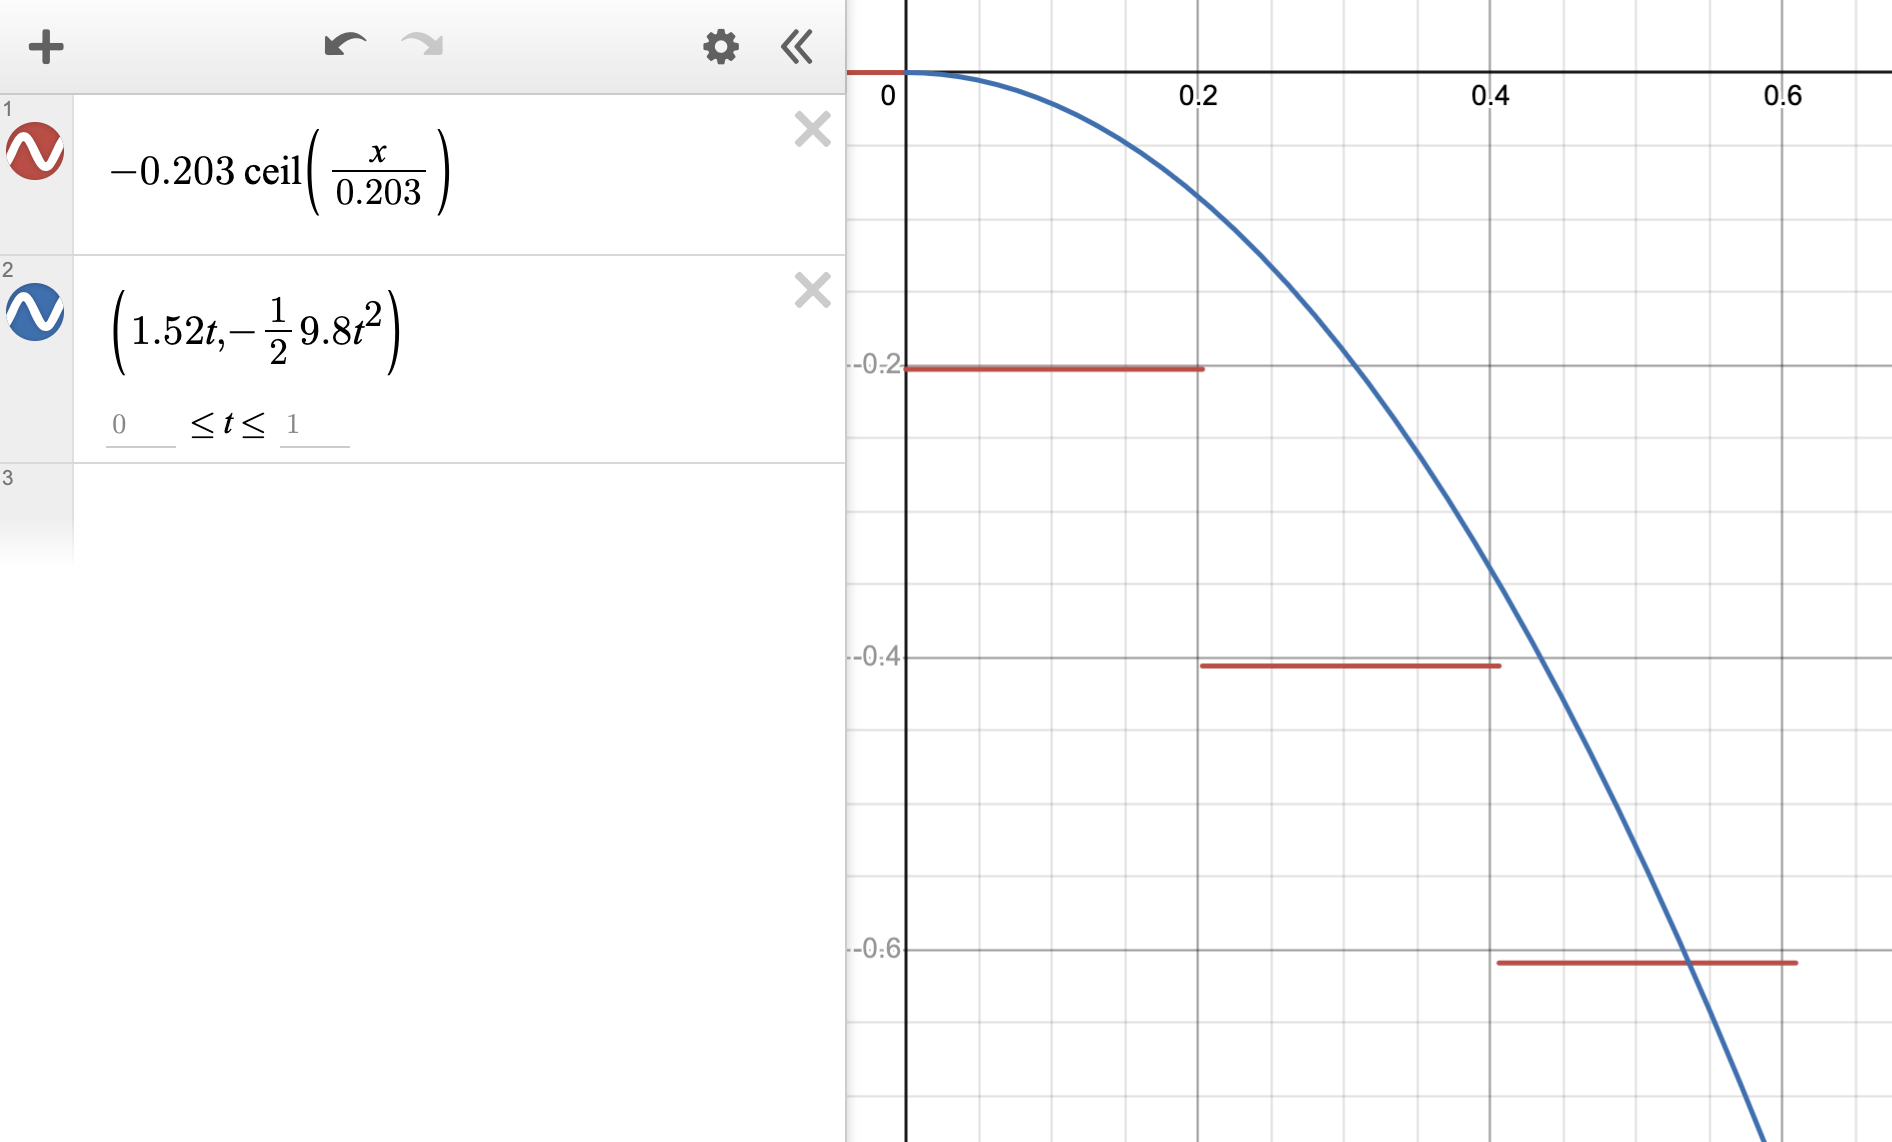
\includegraphics[width=0.7\linewidth]{desmos.png}
    \caption{The ball hits the \fbox{3rd step.}}
    \label{problem4.55}
\end{figure}

\newpage
\subsection{Problem 4.69}
A cameraman on a pickup truck is traveling westward at 20 km/h while he records a cheetah that is moving westward 30 km/h faster than the truck. Suddenly, the cheetah stops, turns, and then runs at 45 km/h eastward, as measured by a suddenly nervous crew member who stands alongside the cheetah’s path. The change in the animal’s velocity takes 2.0 s. 
\begin{figure}[h]
    \centering
    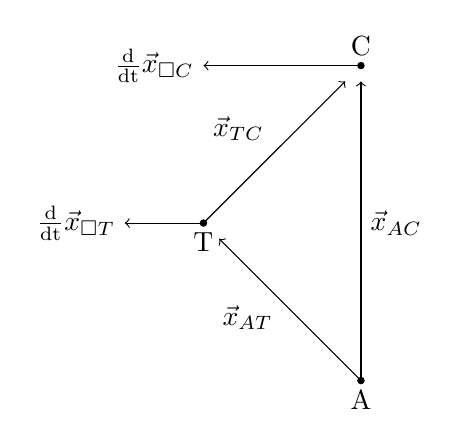
\begin{tikzpicture}[scale=2.0]
        \draw[fill] (0,0) circle[radius=0.02cm] node[below,anchor=north] {A} (-1,1) circle[radius=0.02cm] node[anchor=north] {T} (0,2) circle[radius=0.02cm] node[anchor=south] {C};
        \draw[->] (0,0) -- (-0.9,0.9);
        \draw[->] (-1,1) -- (-0.1,1.9);
        \draw[->] (0,0) -- (0, 1.9);
        \draw (-0.5,0.4) node[anchor=east] {$\vec{x}_{AT}$};
        \draw (0, 1) node[anchor=west] {$\vec{x}_{AC}$};
        \draw (-1, 1.6) node[anchor=west] {$\vec{x}_{TC}$};

        \draw[->] (-1,1) -- (-1.5,1) node[anchor=east] {$\tderiv \vec{x}_{\square T}$};
        \draw[->] (0,2) -- (-1,2) node[anchor=east] {$\tderiv \vec{x}_{\square C}$};
    \end{tikzpicture}
    \caption{The crew member A observing the moving truck T and running cheetah C. The cameraman on the truck T also observes the cheetah C. Although drawn in 2 dimensions for clarity, the problem is worked in only 1 dimension.}
    \label{fig:enter-label}
\end{figure}

We know from the triangle property that $\vec{x}_{AT} + \vec{x}_{TC} = \vec{x}_{AC}$. Because the derivative is a linear operator, the same relationship holds for velocities and accelerations. 

Initially, we know that the cameraman observes a velocity $\tderiv \vec{x}_{TC} = -30\,\si{km/h}$, assuming that the negative direction is west. This corresponds to $\tderiv \vec{x}_{AC}\text{(initial)} = \tderiv \vec{x}_{AT} + \tderiv \vec{x}_{AC} = -50\,\si{km/h}$ observed by the cameraman. The crew member sees the car at $\tderiv \vec{x}_{AT}\text{(initial)} = -20\,\si{km/h}$. 

After the cheetah turns, the crew member observes a velocity $\tderiv \vec{x}_{AC}\text{(final)} = 45\,\si{km/h}$, which corresponds to $\tderiv \vec{x}_{TC}\text{(final)} = \tderiv \vec{x}_{AC} - \tderiv \vec{x}_{AT} = 65\,\si{km/h}$ observed by the cameraman. The fact that we reused the same value for $\tderiv \vec{x}_{AT}$ implies zero acceleration here. Thus, to the cameraman, the average acceleration is:

\[
\vec{a}_\text{avg} = \frac{\vec{v}_\text{final} - \vec{v}_\text{initial}}{\Delta t}
\]
\begin{align*}
\tsderiv \vec{x}_\text{TC} \text{(avg)} &= \frac{\tderiv \vec{x}_\text{TC} \text{(final)} - \tderiv \vec{x}_\text{TC} \text{(initial)}}{\Delta t} =
\frac{(65\,\si{km/h}) - (-30\,\si{km/h})}{2.0\,\si{s}}
\\&\approx{47.5\,\si{km/h^2}}
\end{align*}
The crew member would observe the same acceleration because $\tsderiv \vec{x}_{AT} = 0$, and the triangle relationship holds for accelerations too:
\begin{align*}
\tsderiv \vec{x}_\text{AC} \text{(avg)} &= \frac{\tderiv \vec{x}_\text{AC} \text{(final)} - \tderiv \vec{x}_\text{AC} \text{(initial)}}{\Delta t} =
\frac{(45\,\si{km/h}) - (-50\,\si{km/h})}{2.0\,\si{s}}
\\&\approx{47.5\,\si{km/h^2}}
\end{align*}

\paragraph{A. and C.} Thus, both the cameraman and the crew member observe an acceleration of $\boxed{47.5\,\si{km/h^2}}$, and

\paragraph{B. and D.} They both see that the acceleration is towards the \fbox{east.}


\subsection{Problem 4.97}
A rifle is aimed horizontally at a target 30 m away. The bullet hits the target 1.9 cm below the aiming point. \newline

The bullet's path may be parameterized by 
\[
\vec{x} = \begin{bmatrix}v t \\ -\frac{1}{2} g t^2\end{bmatrix} \qquad g = 9.8\,\si{m/s^2}
\]
At the point of impact, we have
\[
\begin{bmatrix}
    d \\ -h
\end{bmatrix}
= \vec{x}
.\]
We then plug in the values of $d = 30\,\si{m}$ and $h = 0.019\,\si{m}$ and solve for $t$ from the $y$ value, followed by $v$ from the $x$.

\paragraph{A.}
The bullet flies for:
\[
-h = -\frac{1}{2} g t^2
\]
\[
t = \sqrt{\frac{2 (0.019\,\si{m})}{9.8\,\si{m/s^2}}}
\]
\[
t \approx \boxed{0.062\,\si{s}}.
\]

\paragraph{B.}
The bullet leaves the rifle at a velocity of:
\[
vt = d
\]
\[
v = \frac{30\,\si{m}}{0.062\,\si{s}}
\]
\[
v \approx \boxed{482\,\si{m/s}}
\]

\newpage
\section{Other Problems}

\subsection{Miles Driven by Harker}
\begin{figure}
    \centering
    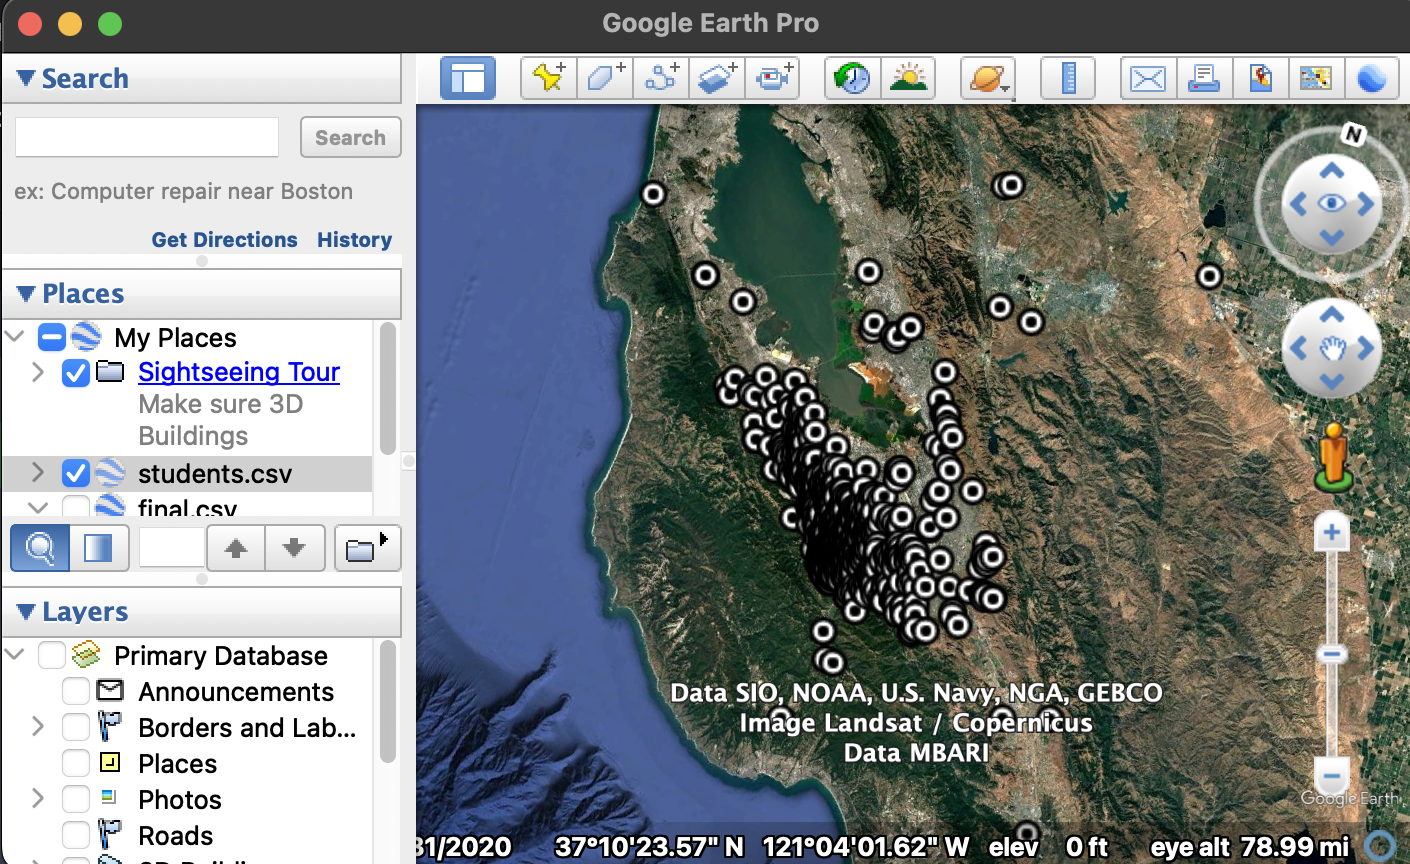
\includegraphics[width=0.7\linewidth]{stalking.png}
    \caption{Stalking the addresses of Harker students.}
    \label{fig:enter-label}
\end{figure}

By downloading the database of addresses on InfiniteCampus, we can calculate the average distance driven by a Harker Upper School student each day. From these data, we get that the average upper school student lives 6.25 miles away from campus (assuming flat Earth). Thus, the number total miles driven per school year is approximately
\begin{align*}
(6.25\,\text{mi per trip per person})\times(2\,\text{trips/day})\times(180\,\text{days/school year})\times(995\,\si{people})\\ = 2.24\times10^6\,\si{mi/year}
\end{align*}

That is equal to \fbox{12.02 light seconds!} Still, this should be a massive underestimate as this only accounts for the straight line distance (ignoring the curvature of the Earth and the fact that one has to drive on roads), and it only accounts for 2 trips per person per day. The figure of 995 people is pulled from the number of people in the Upper School Students Schoology group, and 180 days is the length of a school year for public schools in California. These calculations were done in Mathematica and are in the documentation.

\newpage
\subsection{Cross-sectional Area of Vehicles}

A Honda Civic measures 70.9 in by 55.7 in,\footnote{\url{https://automobiles.honda.com/civic-sedan}} giving a cross-sectional area of $27.42\,\si{ft^2}$. This is a slight overestimate as it does not account for the contour of the car.

For a SUV, an Audi Q7 is 77.6 in by 68.5 in,\footnote{\url{https://www.audilacrosse.com/2023-audi-q7-dimensions.htm}} which is a cross-sectional area of $36.91\,\si{ft^2}$.

For a bicycle and its rider, I will ignore the bicycle as it has a relatively small area compared to its rider, and the area from the rider's thighs probably makes up for it. Thus, I will approximate using half of the ``Body Surface Area,'' which sounds kind of gross and allegedly works out to  $11.09\,\si{ft^2}$ for males from 20-79 years old.\footnote{\url{https://en.wikipedia.org/wiki/Body_surface_area}}

I honestly gave up looking for the height of a CalTrain car, so instead I found that a CSX boxcar for freight trains was 10 feet 8 inches by 13 feet in the worst case.\footnote{\url{https://www.csx.com/index.cfm/customers/resources/equipment/railroad-equipment/}} This works out to an area of $139\,\si{ft^2}$.
% --------------------------------------------------------------
%     You don't have to mess with anything below this line.
% --------------------------------------------------------------
 
\end{document}